\documentclass[a4paper,12pt]{article} % The document class with options
\usepackage[T1]{fontenc}
\usepackage{graphics}
\usepackage{graphicx}
\usepackage{url}

% A comment in the preamble


% Define subsubsubsection command


% Adjust the depth of section numbering
\setcounter{secnumdepth}{4}

\title{The drivers of the level of COVID-19 vaccination in Poland}
\date{May 12, 2024}

\author{
    Tymoteusz Barciński\\
    Ziemowit Głowaczewski\\
    Jakub Bazyluk\\
    Antonina Ślubowska, MD\\
    \\
    Warsaw University of Technology,\\
    Faculty of Mathematics and Information Science
}

\begin{document}
% This is a comment

\maketitle

\begin{abstract}


This study investigates the influence of various independent variables on vaccination rates across municipalities, employing both econometric and machine learning methodologies. Emphasizing statistical inference, our research aims to validate hypotheses pertaining to the vaccination process.

In the econometric approach, linear regression models are initially utilized, integrating feature engineering and selection techniques to handle a multitude of predictors. Addressing nonlinearities, additive models with spline basis expansions are considered, ensuring robustness in model specification. Spatial correlation structures are later incorporated using SARAR models, validated through diagnostic tests such as Moran's I.

Concurrently, the machine learning approach serves to corroborate findings from the econometric model, employing explainable AI to ensure interpretability. Notably, the entire dataset is utilized for model estimation to uphold statistical rigor.

Findings indicate significant correlations between vaccination rates and political views, demographic factors, and spatial context. However, discrepancies between expected and observed correlations prompt further exploration, suggesting nuanced relationships requiring deeper analysis.

Overall, our study provides valuable insights into the complex interplay of factors influencing vaccination rates, offering a comprehensive understanding of the vaccination process across municipalities.

\end{abstract}

\section{Background}	
The COVID-19 pandemic, officially declared by the WHO in March 2020, has deeply affected global society, impacting public health, economics, and social dynamics. Healthcare systems worldwide faced shortages of vital resources, leading to the adoption of restrictive measures like lockdowns and social distancing protocols. While these measures aimed to control the spread of infections, they also disrupted social interactions and economic activities, causing widespread financial losses and job insecurity.
By May 2023, collaborative efforts between scientists and public health campaigners led to the development and deployment of effective vaccines, signaling the official end of the pandemic. Despite this milestone, the lessons learned from addressing COVID-19 vaccine hesitancy remain relevant. Vaccine hesitancy, once a significant challenge, may resurface in future, underscoring the need to understand its determinants for preparedness and response efforts in the years to come.
Positioned in Central and Eastern Europe, Poland offers a unique context for studying vaccination behavior, often overlooked compared to more extensively studied regions like the US and UK. Poland's historical experiences, socio-cultural dynamics, and political landscape significantly shape public health policies and vaccination strategies. Furthermore, analyzing regional disparities in vaccination rates within Poland can provide insights into the impact of socio-economic factors, healthcare infrastructure, and access to healthcare services. Despite the availability of COVID-19 vaccines, Poland has shown lower vaccination rates compared to the EU average, underscoring the importance of understanding the underlying reasons for this hesitancy. \cite{covid_vaccine_tracker}
By thoroughly examining these factors, policymakers and healthcare professionals can develop targeted interventions to effectively address vaccine hesitancy and enhance public health outcomes.

\section{Literature review}
To contextualize our study, we conducted a literature review to explore existing research on COVID-19 vaccination acceptance and hesitancy, aiming to understand the various approaches and findings in this area.
\\
\\
The study \cite{vaccines11030700} aimed to assess the factors influencing COVID-19 vaccination acceptance among the Polish population, analyzing sociodemographic factors and physical and mental health status. The evaluation was conducted through a survey involving 200,000 participants from Poland. Logistic regression analysis was employed to identify significant associations between these factors and vaccine acceptance or refusal. The research identified fear of post-vaccination complications and safety concerns as primary reasons for vaccine hesitancy. Male respondents with lower education levels exhibited more negative attitudes, while older individuals, those with higher education, and residents of larger cities were more likely to accept vaccination. Good physical and mental health conditions were also associated with vaccine acceptance.
\\
\\
Another research \cite{vaccines10040528} examined the predictors of delayed COVID-19 vaccine uptake in Polish sub-regions using regression models. Regression analysis was employed to explain the increase in COVID-19 vaccination rates across 378 Polish sub-regions. The analysis compared vaccination rates for age groups of 20 years and older between June 30, 2020, and January 31, 2021. The results indicate that initial high vaccination rates did not reduce willingness to vaccinate, but rather increased it, leading to greater disparities between regions. Support for Eurosceptic and anti-establishment parties strongly correlated with persistent vaccine hesitancy. Social inclusion markers like voter turnout and employment rate remained significant predictors, while higher education levels showed mixed effects on vaccination rates across different age groups. These findings suggest that vaccine hesitancy in Poland is influenced by political views, social exclusion, and regional historical context, rather than anti-vaccine movements.
\\
\\
One approach to assess the various factors contributing to vaccine hesitancy is through the application of psychological concepts like the 5C framework. This model identifies five key factors—confidence, complacency, convenience, risk calculation, and collective responsibility—that influence individuals' decisions regarding vaccination. \cite{10.1371/journal.pone.0208601}, \cite{Machingaidze2021} The study \cite{RANCHER2023180} explored COVID-19 vaccine hesitancy using the 5C model across a national and South Carolina sample. Analyzing data from a national sample (n = 1634) and a South Carolina sample (n = 784), the study investigates how the 5C drivers of vaccine behavior influence early adoption and intentions. Results reveal that the South Carolina sample exhibits lower vaccine intentions and higher levels of 5C barriers compared to the national sample. Moreover, demographic factors such as race and key drivers like confidence and collective responsibility significantly impact vaccine trust and intentions across both groups. 
\\
\\
In our solution, we incorporate insights drawn from the literature review to tackle COVID-19 vaccine hesitancy and boost vaccination rates.


\section{Aim of the study}
Our study aims to investigate the factors influencing COVID-19 vaccination rates at the municipal level in Poland. By analyzing vaccination data alongside socio-demographic, economic, and healthcare-related characteristics of municipalities, we seek to adapt the 5C model to formulate hypotheses about the municipality-level drivers of vaccination uptake. Additionally, we have developed hypotheses not directly related to the 5C components, considering factors such as population density, urban/rural classification, historical partition terrain, and income per capita, as well as spatial dependencies.
\subsection{Hypotheses}
\subsubsection{5C-based hypotheses}
\subparagraph{Confidence}
This component refers to trust in the effectiveness and safety of vaccines, as well as in the healthcare system and authorities that promote vaccination. Factors that can affect confidence include misinformation, mistrust in healthcare providers or pharmaceutical companies, and concerns about vaccine side effects.
\\
As a potential measure of general trust in authorities, we considered the percentage of participants in parliamentary elections. Additionally, we investigated the voting patterns of residents in each municipality.
\\
We hypothesized that a higher voter turnout correlates with a higher vaccination rate, and that political affiliation impacts vaccination acceptance rates. 
\subparagraph{Complacency}
Complacency refers to the perception of the risk posed by vaccine-preventable diseases. When individuals perceive these diseases as low-risk or non-threatening, they may become less inclined to get vaccinated.
\\
Due to the increased risk that elderly individuals face from developing severe forms of COVID-19 and related complications, they exhibit greater willingness to receive vaccinations. Moreover, vaccination programs often prioritize this demographic. 
\\
Consequently, our hypothesis suggests that municipalities with a higher proportion of seniors will exhibit higher vaccination rates, while those with a higher proportion of individuals under the age of 20 will likely demonstrate lower vaccination rates.

\subparagraph{Convenience}
Convenience refers to the ease of access to vaccination services. Barriers to vaccination, such as long wait times, inconvenient clinic hours, or lack of transportation to vaccination sites, can reduce vaccine uptake. 
\\
Based on this, we hypothesize that the number of cars per 1000 inhabitants will positively correlate with vaccination rates. 
\\
Additionally, we obtained data on the number of vaccination sites situated within a 10-kilometer radius of the municipality's center and minimal distances from the center of the municipality to the nearest vaccination point in March 2021, at the outset of the vaccination campaign. We regarded these factors as indicators of the intensity of vaccination efforts within each municipality. 
\\
Our hypothesis posited that these factors would positively correlate with the final vaccination rate in 2021.


\subparagraph{Risk calculation}
Calculation refers to the process individuals use to weigh the risks and benefits of vaccination. Factors influencing this calculation include perceived vaccine efficacy, perceived severity of vaccine-preventable diseases, and perceived risk of vaccine side effects. Individuals may be more likely to accept vaccination if they perceive the benefits of vaccination to outweigh the risks.
\\
Based on this understanding, we hypothesize that a higher percentage of residents with higher education levels will positively correlate with vaccination rates. This assumption stems from the notion that education fosters a better understanding of the benefits of vaccination, thereby increasing acceptance rates.

\subparagraph{Collective responsibility}
Collective responsibility refers to the sense of duty individuals feel towards protecting the health of their community through vaccination. Factors influencing collective responsibility include social norms surrounding vaccination, perceived social pressure to vaccinate, and the belief that vaccination is a civic duty. Strengthening collective responsibility can help foster a culture of vaccination acceptance.
\\
This concept intersects with the hypotheses outlined in section 3.1.1.

\subsubsection{Other factors}
In addition to examining the 5C components, our study aimed to explore how the diverse characteristics of Polish municipalities relate to vaccination rates. These characteristics include population density, urban or rural classification, historical partitions of Poland's terrain, and income per capita, reflecting the economic diversity across Poland's regions.
\\
Our hypothesis suggests that all of these factors play a role in shaping vaccination rates. Particularly, we anticipate a positive correlation between income per capita and vaccination rates, as higher income levels often improve access to vaccination services, thereby enhancing convenience aspect mentioned in 3.1.1.3.
\\
\\
Last but not least, we decided to verify whether the vaccine acceptance in a municipality's neighborhood affects the vaccination rate in the municipality itself. Intuitively, we formulated the hypothesis that these factors should be related, even after controlling for all other significant variables.

\newpage
\subsection{Summary}
All hypotheses are summarized in the table below.
\begin{table}[htbp]
    \centering
    \caption{Summary of Hypotheses}
    \scalebox{0.85}{
    \begin{tabular}{|c|p{13cm}|}
    \hline
    \textbf{Hypothesis} & \textbf{Description} \\
    \hline
    H1 & Higher voter turnout correlates with a higher vaccination rate.  \\
    \hline
    H2 & Political affiliation impacts vaccination acceptance rates. \\
    \hline
    H3 & Municipalities with a higher proportion of seniors exhibits higher vaccination rates, while those with a higher proportion of individuals under the age of 20 likely demonstrates lower vaccination rates. \\
    \hline
    H4 & Municipalities with a higher proportion of seniors exhibits higher vaccination rates. \\
    \hline
    H5 & Intensity of vaccination efforts at the outset of the vaccination campaign positively correlates with the final vaccination rate in 2021.\\
    \hline
    H6 & Higher percentage of residents with higher education levels will positively correlate with vaccination rates. \\
    \hline
    H7 & Population density, urban or rural classification, historical partitions of Poland's terrain, and income per capita play a role in shaping vaccination rates. There is a positive correlation between income per capita and vaccination rates.\\
    \hline
    H8 & Vaccine acceptance in a municipality's neighborhood affects the vaccination rate in the municipality itself, even after controlling for all other significant variables.\\
    \hline
    \end{tabular} 
    }
    \label{tab:Final hypotheses }
\end{table}

\newpage
 
\section{Data preparation}

\subsection{Data provided by the Warsaw Econometric Challenge organizers}
The organizers provided datasets with information about polish municipalities (describing the situation in 2021) and counties (describing the situation in 2020). The data revolves around the percentages of vaccinated population and socio-economic situation of given locations. Moreover, spatial mapping of said municipalities and counties was provided, with an addition of potential historical / geographical divisions -- the map of partitioned Poland and east-west split.

\begin{table}[htbp]
  \begin{tabular}{|l|l|}
    \hline
  Name of data file        & Year of measurement \\
  \hline
  data\_municipalities.csv & 2021                 \\
  data\_counties.csv       & 2020      \\        
  \hline 
  \end{tabular}
\end{table}

 
\subsection{Additionally acquired data}
Shape files for municipalities and historical partitions of Poland
Dataset about the 2019 parliamentary election results by municipality from the National Elections Committee.
Dataset about vaccination points in Poland from 09-03-2021. \cite{polonszczepien2021}

 
\subsection{Dependent variable}
The \texttt{\mbox{percent\_vaccinated}} is a variable whose dependencies are studied in this paper. It is showing the percentage of vaccinated population per municipality. On the national level, we can observe that the variable displays a significant variance depending on location of the measurement. Furthermore, basing on papers on the topic, \cite{dolman2023opposing} 
it is observed that political affiliation is a strong predictor of a person's willingness to vaccinate.
 

\subsection{Variables description}
In our municipality-wise analysis, we used the following variables:

\begin{itemize}
    \item \texttt{voters\_turnout} - Per municipality percentage voter turnout
    \item \texttt{SLD\_percent}, \texttt{PO\_percent}, \texttt{Konfederacja\_percent}, \texttt{PSL\_percent} - Percentage results of Polish 2019 Parliamentary elections for the opposition parties per municipality
    \item Logarithm of \texttt{revenues\_per\_capita\_PIT} - Logarithm of national budget in income tax revenues from the given municipality
    \item \texttt{percent\_over\_60} - Percentage of municipality population above 60 years old
    \item Square root of \texttt{min\_dist} - Square root of minimum distance to a vaccination point from the given municipality in kilometers
    \item \texttt{no\_loc\_in10km} - Number of vaccination points within a 10-kilometer radius from the municipality
    \item \texttt{education\_share\_higher} - Percentage share of population with higher education
    \item \texttt{healthcare\_advices\_ratio\_total} - Number of healthcare advices provided per capita
    \item Second degree polynomial transformation of \texttt{cars\_per\_1000\_persons} - Number of cars per 1000 capita
\end{itemize}

\subsection{Features Understanding}

\begin{itemize}
    \item \texttt{political\_variables} - From available scientific sources, we deduced that political views and local political engagement are important factors in personal attitudes towards vaccination.
    \item Logarithm of \texttt{revenues\_per\_capita} - We decided that income tax revenue is a good metric of a municipality's economic situation, which correlates with willingness to vaccinate.
    \item Similar correlation occurs with \texttt{education\_share\_higher} and\\ \texttt{healthcare\_advices\_ratio\_total} - Predictors of belief in scientific and medical methods, resulting in an inclination towards vaccination.
    \item Variables relating to spatial relations of municipalities to vaccination points - \texttt{no\_loc\_in10km}, \texttt{min\_dist}, and \texttt{cars\_per\_1000\_persons} are metrics of vaccination availability in given locations, and capabilities to reach said locations.
\end{itemize}


\newpage
\section{Methodology}
The effect of independent variables on the $\texttt{percent\ vaccinated}$ for each municipality was modelled by two different approaches. Firstly, the econometric approach based on the linear models, which was later extended to take into account the spatial correlation structure between observations, and secondly the machine learning approach. Note, that the emphasis in this study is on the statistical inference to draw conclusions related to the hypothesis list. Therefore, the machine learning approach is included to confirm or reject the conclusions drawn from the linear model based on the statistical tests, via the explainability artificial intelligence. Moreover, since the goal was statistical inference, the dataset was not divided into the training and testing parts, but the entire dataset of all municipalities was used for model estimation.

The dependent variable $\texttt{percent\ vaccinated}$ proposed by the organizers was bounded between zero and one hundred. We decided to transform the variable via the logit function after dividing it one hundred. This allows the new dependent variable to be unbounded which doesn't violate the assumption of the linear model.


\section{Econometric approaches}

\subsection{Linear model}
\subsubsection{Approach}
Linear models are widely used in many different areas of modelling due to interpretability and inference. In our study we used linear regression modelling approach to allow for the statistical inference on coefficients. Due to the high number of potential predictors after extensive feature engineering, feature selection methods were used. The forward and backward feature selection methods were utilized, which allowed for initial diagnostics of significant predictions. Moreover, linear Pearson correlation between independent variables and the dependent variable was considered. After a subset of predictor was chosen, the modelling approach focused on adding new variables to the linear model in an interative fashion. The nonlineartites were dignozed and accounted for by the usage of the partial residual plots. Moreover, the additive models with spline basis expansions were considered to detect potential nonlinearities, \cite{wood2017generalized} which were later parameterized and included in the linear model (such as via the square root, logarithm or quadratic expansion). Importantly, the variables that related to our hypothesis were chosen. Note that those variables were not dropped in the model reduction phase, which was performed via the F tests, because of their significance for stated hypothesis. 

\subsubsection{Results}

Details of the estimated linear regression model are presented in \ref{fig:coefficients_regression_simple}. The variables related to the political views were found to be significant. The PIS\_percent variable was excluded from the model due to high correlation with the variable PO\_percent (-0.88). Spatial variables related to partitions and municipality type are also significant, and almost all of them (except for mixed municipality type) contribute positively to the vaccinated percent.

The function of form of some independent variables included in the model are seen in the partial residual plots in the figure \ref{fig:partial_residuals_effects}. It can be visually identified that the coefficients estimated by the linear model are sensible.

The assumptions of the linear model were verified. The figure \ref{fig:diagnostics_mvp} shows the standard diagnostics plots. By visual diagnostics, we see the heavy tails of the residuals from the QQ plot, but apart from that no serious validations of the linear models assumptions are reported. The lack of multicolinearity between the independent variables were confirmed by the Varaince Inflation Factor shown in figure \ref{fig:vif_mvp}. The model does not take the spatial dependence into account so the spatial correlation of the residuals were investigated, initally by the map shown in figure \ref{fig:res_linear}. We clearly see the spatial dependence of residuals in certain parts of Poland. This dependence was confirmed by the Moran’s I test with the $p values \leq 0.001$. Therefore the assumptions of the linear model are not fully satisfied and it motivates us to consider tha spatial regression models in the subsequent section.

\begin{figure}[htp]
    \centering
    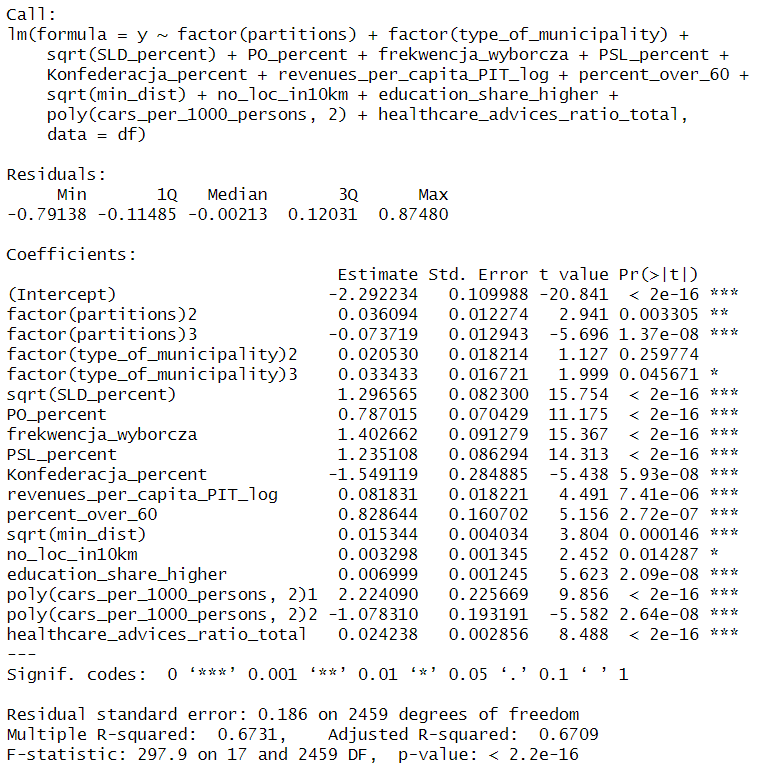
\includegraphics[width=0.9\textwidth]{assets/coefficients_regression_simple.png}
    \caption{The estimated linear regression models with summary statistics and p values of statistical t tests on the coefficients}
    \label{fig:coefficients_regression_simple}
\end{figure}

\begin{figure}[htp]
    \centering
    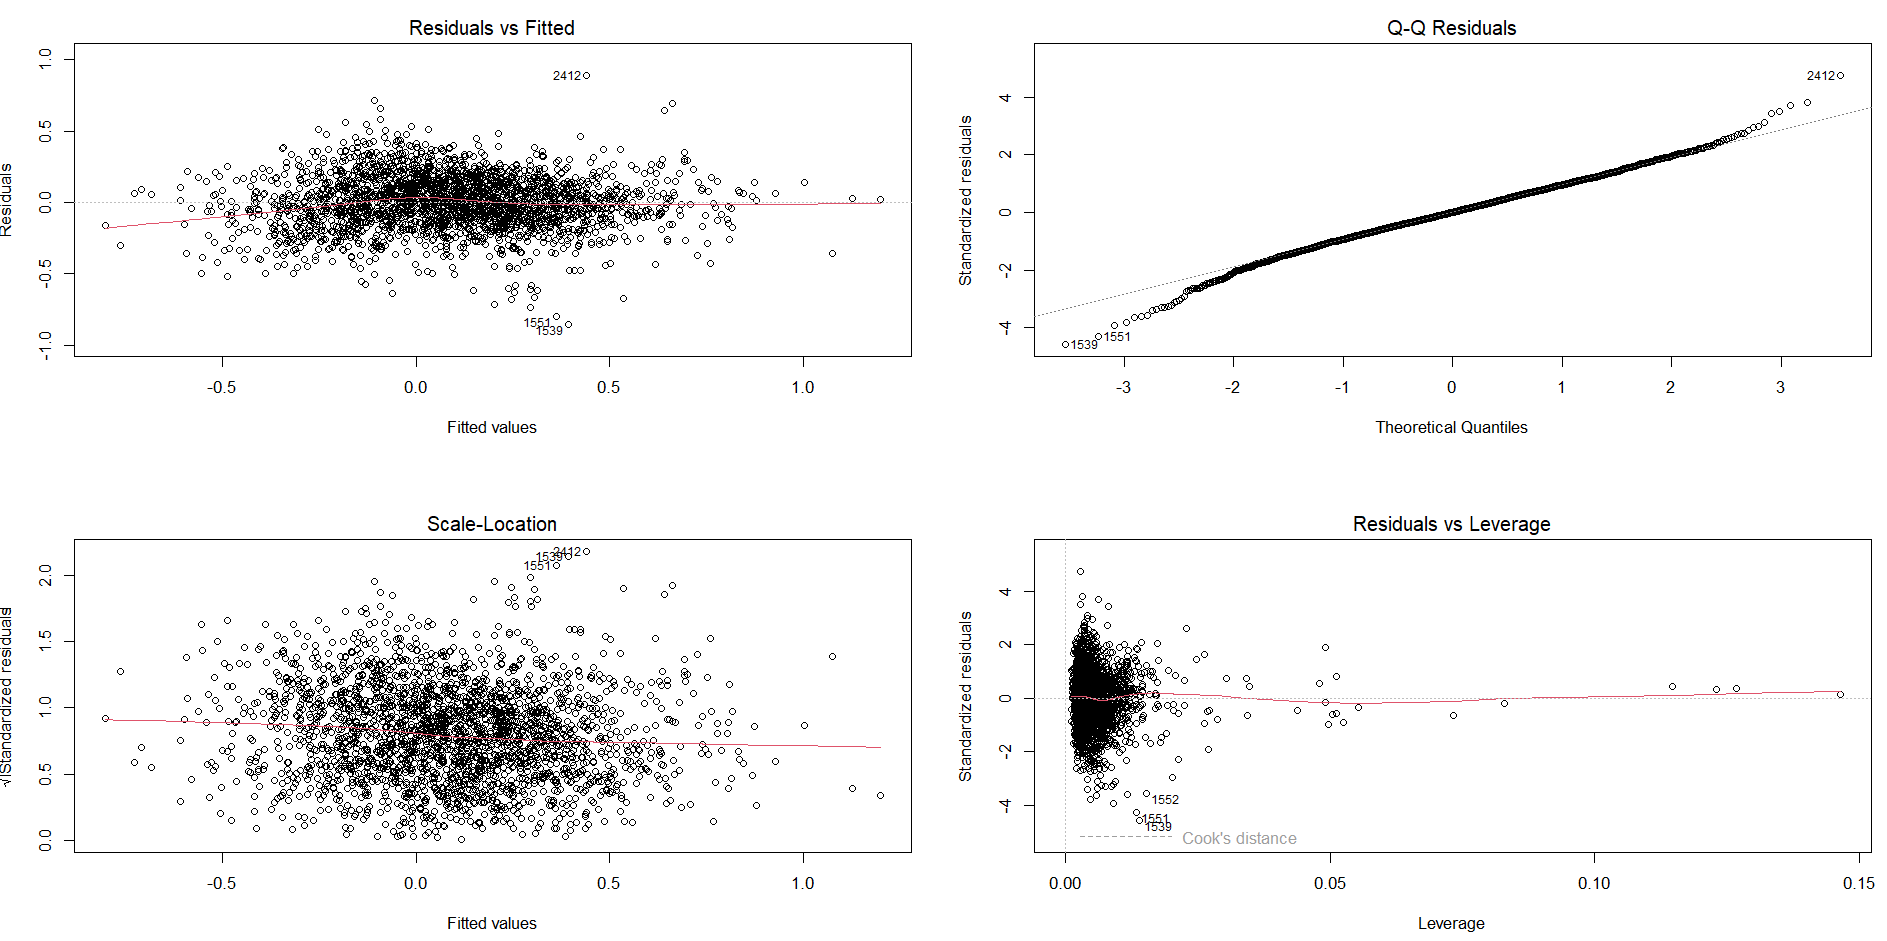
\includegraphics[width=1\textwidth]{assets/diagnostics_mvp.png}
    \caption{The diagnostics plot for the estimated linear regression model, indicating no significant violation of the model assumptions}
    \label{fig:diagnostics_mvp}
\end{figure}

\begin{figure}[htp]
    \centering
    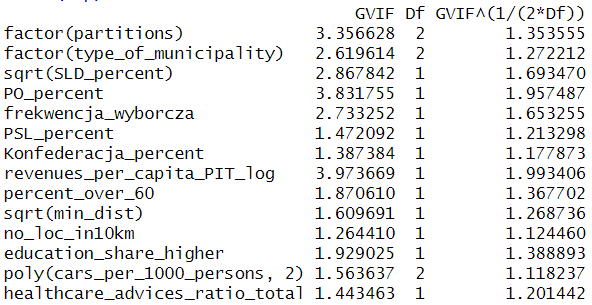
\includegraphics[width=0.8\textwidth]{assets/vif_mvp.png}
    \caption{The Variance Inflation factor for included variables in the linear model}
    \label{fig:vif_mvp}
\end{figure}

\begin{figure}[htp]
    \centering
    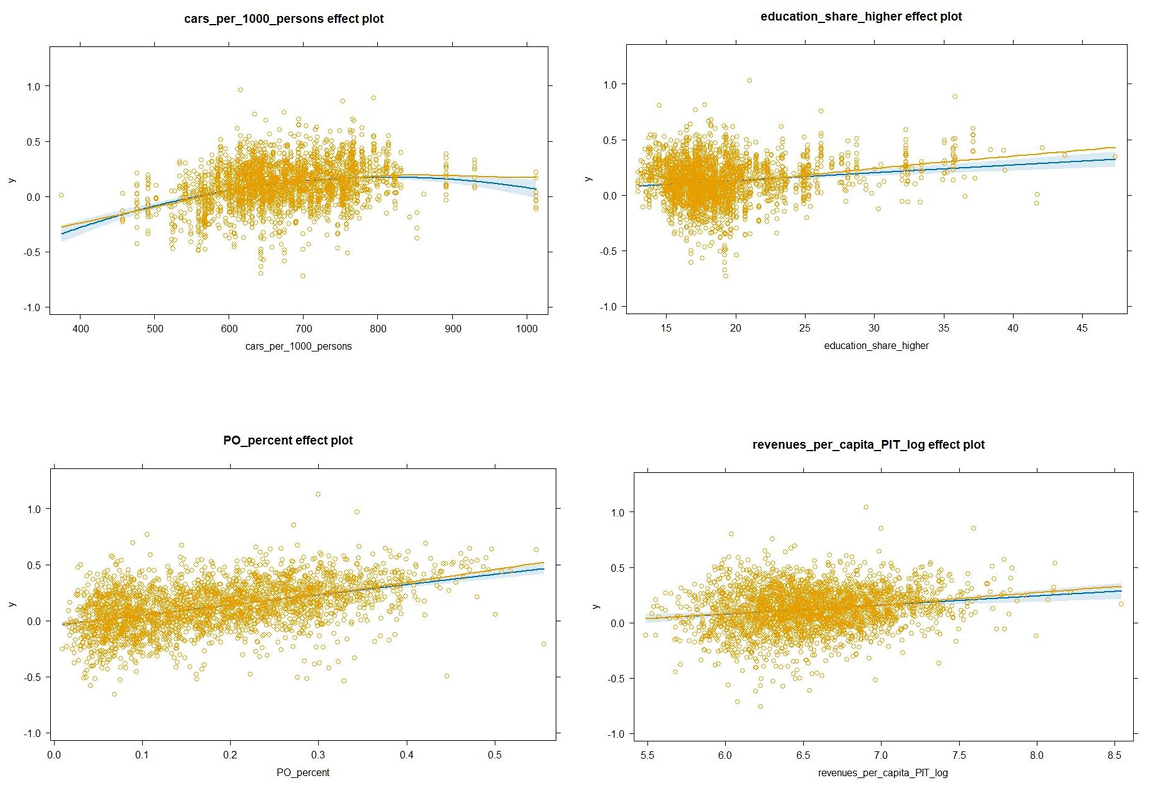
\includegraphics[width=1\textwidth]{assets/partial_residuals_effects.png}
    \caption{Partial residual plots between the selected independent variables and the partial residuals, which indicated the validity of the function form of selected 
    independent variables in the regression model}
    \label{fig:partial_residuals_effects}
\end{figure}

\begin{figure}[htp]
    \centering
    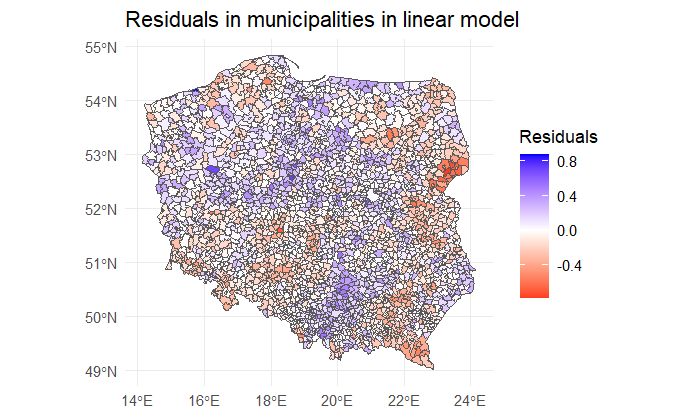
\includegraphics[width=1\textwidth]{assets/res_linear.png}
    \caption{Residuals of the linear model across space, clear indication of spatial dependence structure are present}
    \label{fig:res_linear}
\end{figure}

\begin{figure}[htp]
    \centering
    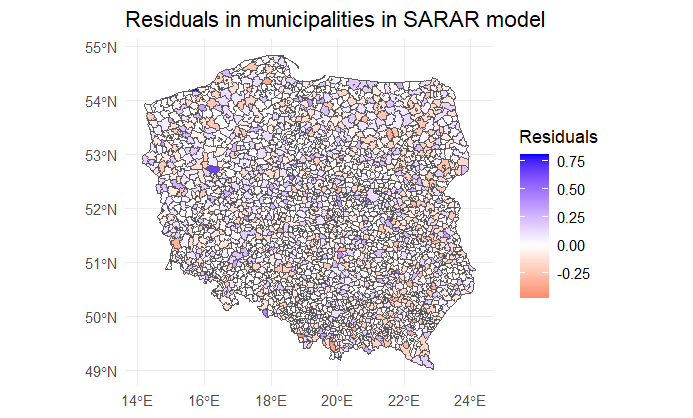
\includegraphics[width=1\textwidth]{assets/res_sarar.png}
    \caption{Residuals of the spatial linear model across space, indicating that no spatial dependence structure}
    \label{fig:res_sarar}
\end{figure}

\newpage
\subsection{Econometric approach with spatial dependence }

\subsubsection{Approach}

\begin{figure}[htp]
    \centering
    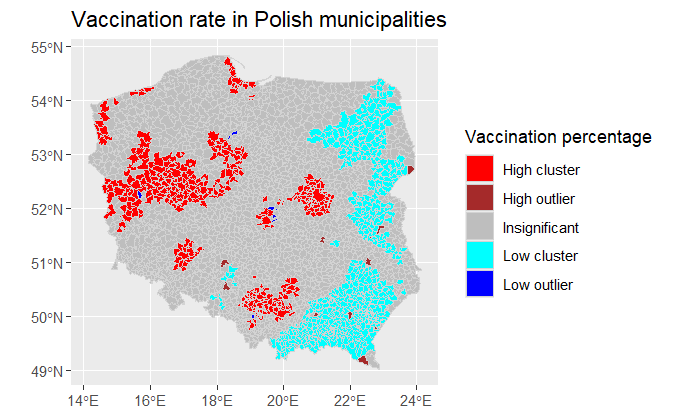
\includegraphics[width=1\textwidth]{assets/vaccination_rate.png}
    \caption{The diagnostics plot for the estimated linear regression model, indicating no significant violation of the model assumptions}
    \label{fig:LISA method}
\end{figure}
SAC/SARAR models are used in cases where the spatial dependence of dependent variable is  significant. Based on previous models it is a sensible hypothesis. First, we applied LISA method to visually analyze map of dependence \ref{fig:LISA method}. In order to formally check the presence of spatial dependence and thus proving our approach reasonable we performed Moran's I test. We obtained Moran I statistic 0.71, which was enough to reject the hypothesis of independence with p-value < 2e-16.  We decided to incorporate spatial component into our analysys using Spatial Autoregressive with Autoregressive Conditional Heteroskedasticity (SARAR) model. \cite{bivand2013applied}

\subsubsection{Model formulation}

Model is given by following equation:

\[y = \rho_{Lag}W y + X\beta + u, \quad u = \lambda _{Err}Wu + \epsilon\]

\newpage
\noindent Where:

$y$ - dependent variable percent vaccined

$\rho_{Lag}$ - spatial autoregressive coefficient

$W$ - matrix of weights

$ \lambda _{Err}$ - spatial moving average coefficient

$ \epsilon \sim N(0,\sigma^2)$

Parameters $\rho_{Lag}$, $ \lambda _{Err}$ and $\beta$ are estimated using MLE and $W[i,j]$ is reversed distance between municipalities $i$ and $j$ for $i \neq j$ and $W[i,i] = 0$. Distance is calculated using Hervesine formula for exact real-life distances between municipalities. We then proceeded to perform another Moran I test for residuals obtaining Moran I statistic $= -0.05$ and $p-value = 0.9999$. Therefore there is no reason to assume that residuals in our model are spatially dependent, consequently proving that our model was properly chosen. 

\subsubsection{Results}

The conditional component accounts for additional predictors that may influence vaccination percent, such as population demographics, healthcare infrastructure, and socioeconomic factors.  The error component captures unobserved factors and measurement error that contribute to variability in vaccination percent. Spatial autocorrelation in the errors is accounted for, indicating that errors in vaccination percent for neighboring municipalities may be correlated. The SAC/SARAR model allows for the interpretation of coefficients representing the direct effects of predictors on vaccination percent, excluding spatial effects. These were covered by the model and are not present in coefficients due to model architecture. This was confirmed by the model that included factors of partitions (relating to geopolitical partitions of Poland during XIX century) and municipality factor (rural, urban and mixed). All of them turn out to be insignificant, which is astounding result, once again proving that our approach is well-chosen.

Finally we prepared map of residuals similar to previous models \ref{fig:res_sarar} that is clearly interpretable. Residuals are actually random in space. Residual in linear model map have clear dependence, see \ref{fig:res_linear} for comparison.


\newpage
\section{Machine Learning Approach}
\subsection{Motivation and approach}

We have trained a machine learning model to see if potential complex non-linear dependencies change the impact of predictions on our target variable. We have used XGBoost model, because it proves to be effective solution for tabular data. \cite{10.1145/2939672.2939785} We have trained it on the same data that we used with linear model, however we did not apply any transformations to it (apart from one-hot-encoding of categorical variables), because we wanted the model to figure it out by itself. We do not compare performance of ML model with linear model, because we do this analysis only for explainability purposes. 

Explanation of this model was done using SHAP analysis: SHapley Additive exPlanations. SHAP values are a method used in machine learning to explain the prediction of a model by quantifying the contribution of each feature to the prediction. They provide insights into how each feature affects the model's output, helping understanding model behavior and feature importance. \cite{Lundberg2017AUA}

SHAP analysis provides us with a SHAP value for each feature of each observation in our dataset. SHAP value measures how value of given feature in given observation “moves” our prediction away from baseline prediction (which is usually average of all predictions in our dataset). This can be represented on a “beeswarm plot”, where SHAP values are represented on the x-axis, while the y-axis represents the features. Each observation in the dataset is then represented as a point on the plot, with the color of the points representing the value of the corresponding feature. This visualization helps to understand how the SHAP values vary across different features for each observation in the dataset.


\newpage
\subsection{Results}
Beeswarm plot of our XGBoost model is presented in Figure \ref{fig:beeswarm} below.
\begin{figure}[htbp]
    \centering
    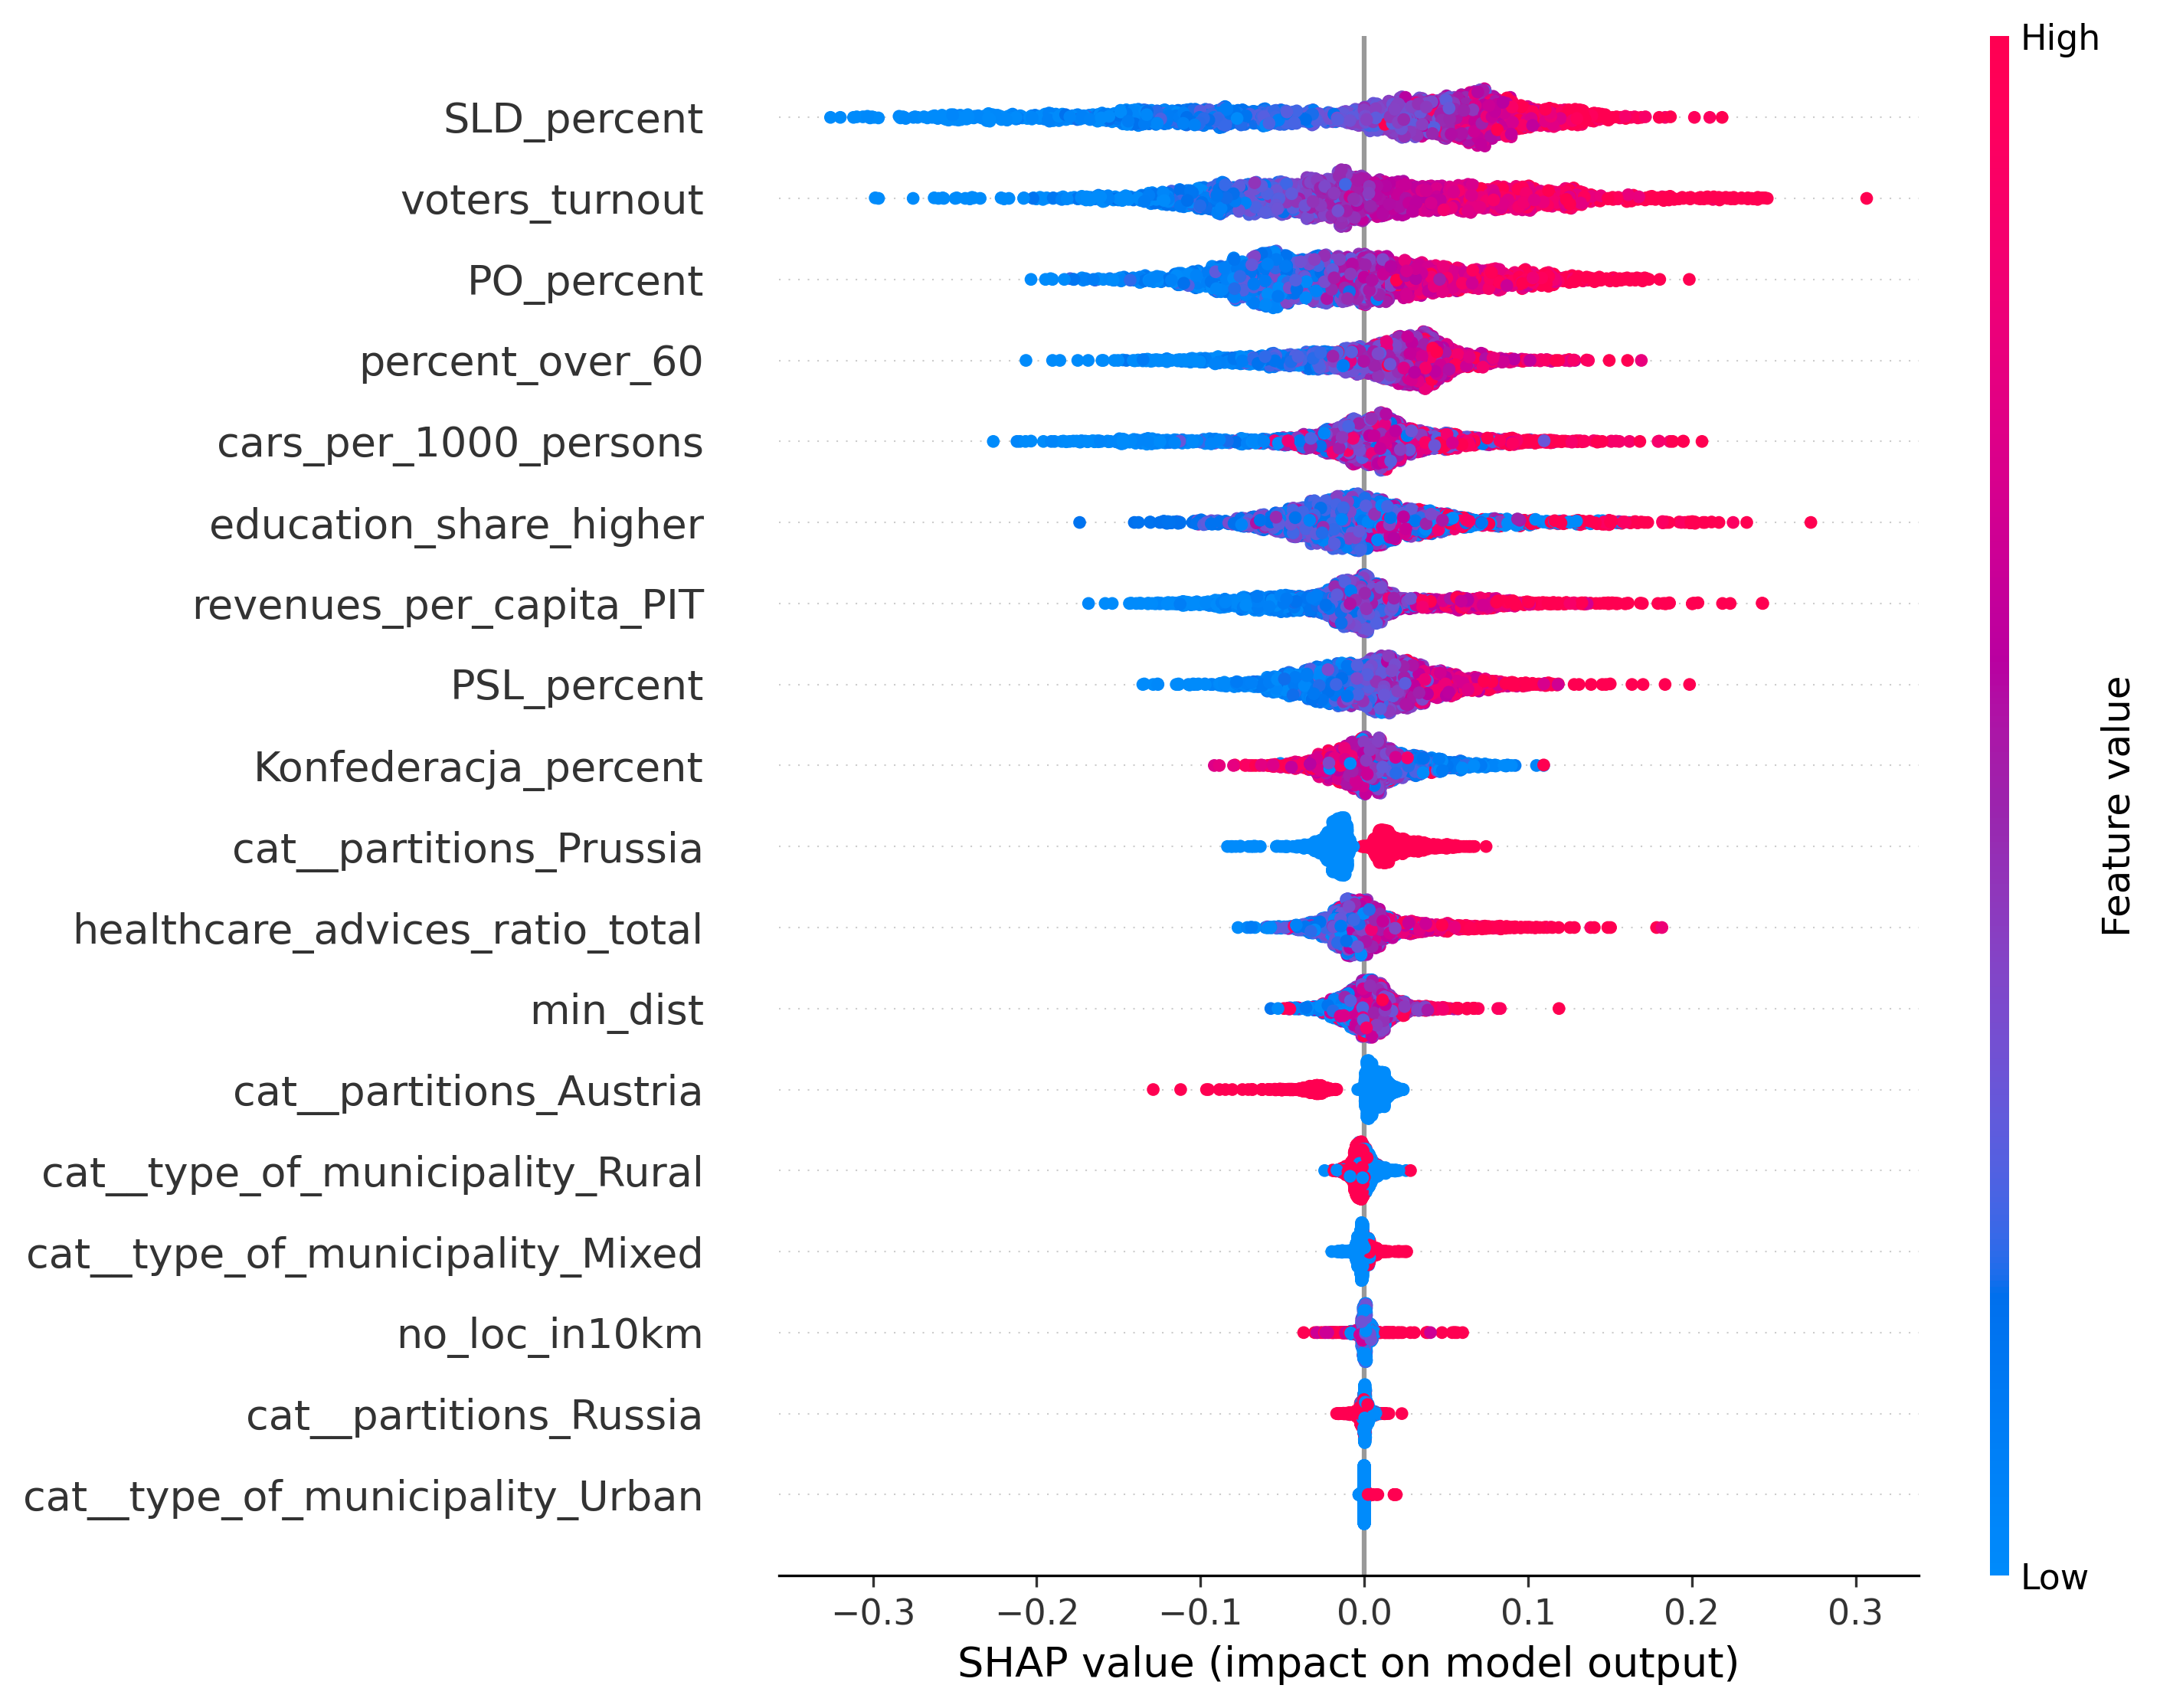
\includegraphics[width=0.8\textwidth]{assets/beeswarm.png}
    \caption{Caption of the beeswarm plot}
    \label{fig:beeswarm}
  \end{figure}

  As we can see, explain ability results from XGBoost model are similar to ones we have observed in the linear model. The beeswarm plot analysis reveals a consistent alignment between the interpretability results obtained from the XGBoost model and the observations derived from the linear model. Notably, key factors driving vaccination rates in Polish municipalities predominantly stem from political and educational variables.

  Leading the pack are variables associated with political affiliations and participation, such as voters turnout, and percentages of votes for parties indicating their substantial influence on vaccination outcomes. We can also see that political affiliations are in line with expectations: votes for parties that are considered progressive (SLD and PO) have positive impact on vaccination rates, while for conservative party (Konfederacja) has negative impact. PSL party, generally conservative (but as of 2024 in coalition with SLD and PO) also has positive impact on vaccination rates. 
  
  Interestingly, we can see that the relationship between each feature and its SHAP value appears more condensed compared to the typical scatterplot distribution observed between features and predictions. Instead of a scattered cloud of points, the SHAP values exhibit a more concentrated pattern resembling a function plot, where for a given X, the associated SHAP values cluster closely around a singular Y value, which is especially visible for political parties as seen in the Figure \ref{fig:parties_partial} below. 
  

  \begin{figure}[htbp]
    \centering
    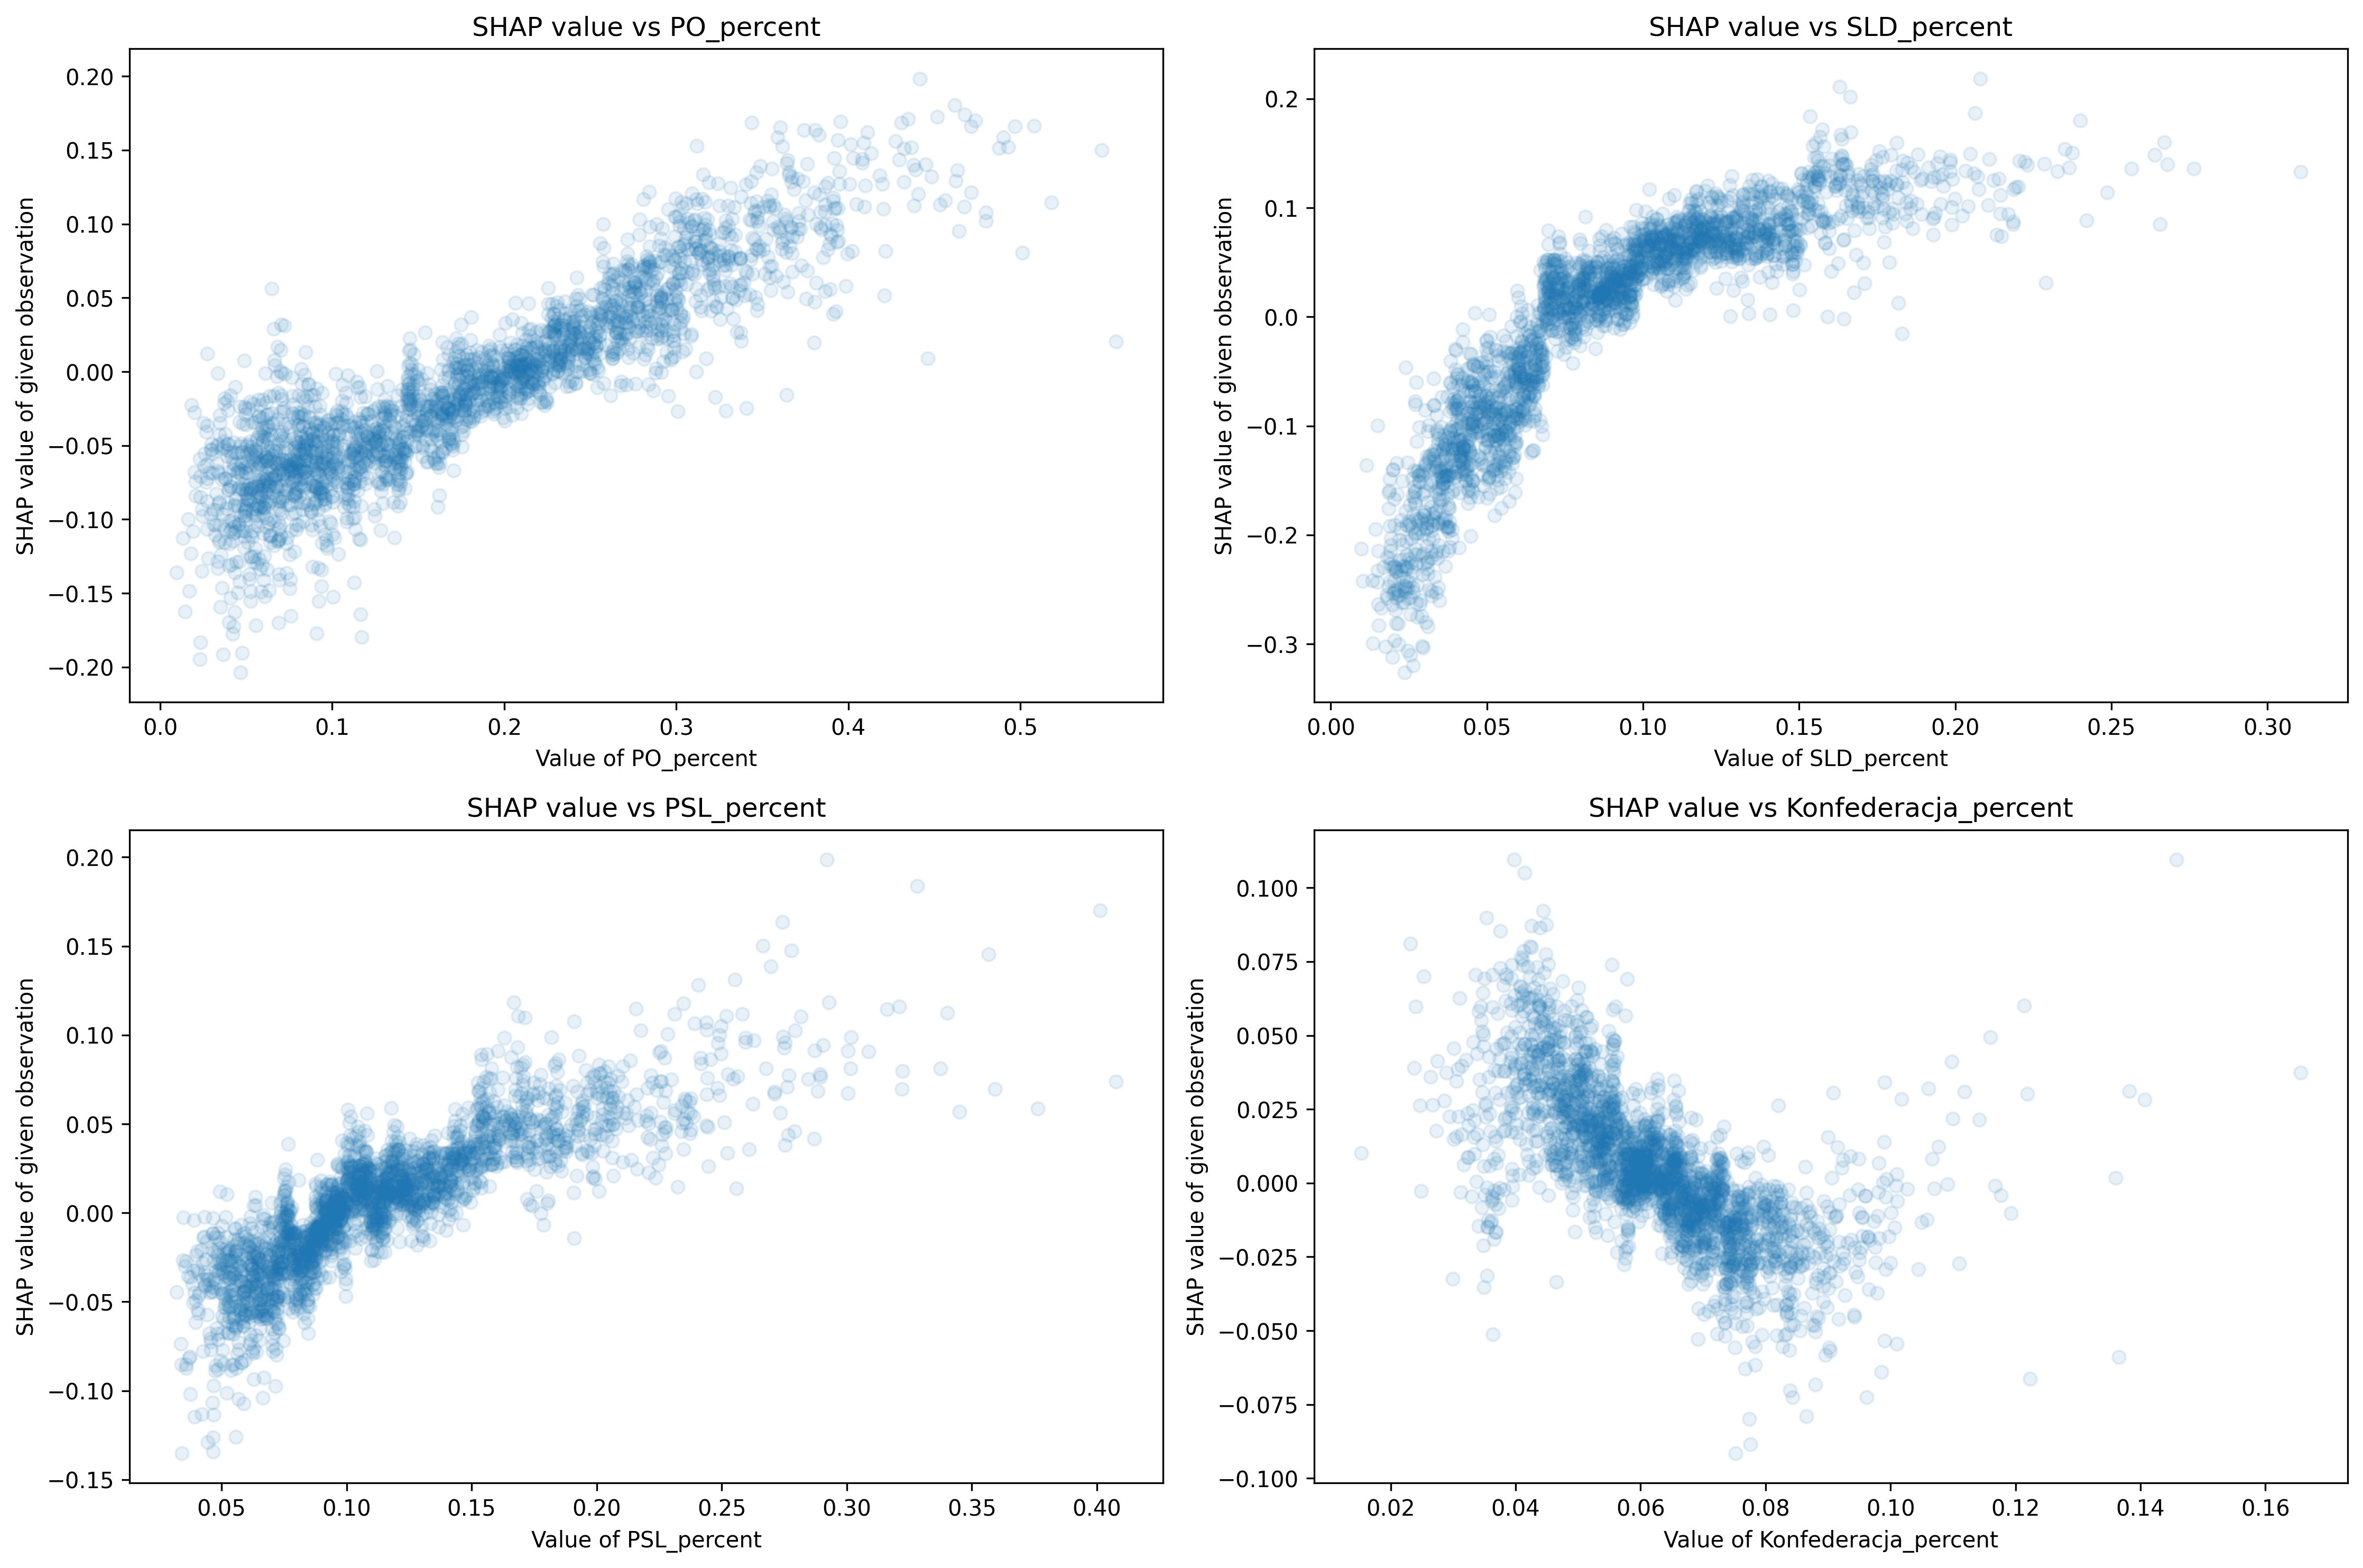
\includegraphics[width=1\textwidth]{assets/parties_partial.png}
    \caption{Caption of the beeswarm plot}
    \label{fig:parties_partial}
  \end{figure}

  Demographic characteristics also play a discernible role, with variables like percentage of people over 60 and cars per 1000 persons highlighting the influence of age distribution and accessibility on vaccination uptake. However, certain features exhibit relatively lower importance, such as type of municipality, suggesting their minor impact on vaccination rates within the studied context.

We can see that historical partitions of Poland have generally have impact in line with our expectations (negative for Austrian and positive on Prussian), however that impact is low. We believe that this is caused by high correlation between historical partitions and other variables that are already included in the model. 

The consistent alignment between the XGBoost and linear model results validates the pivotal role of political and educational variables in shaping vaccination rates across Polish municipalities. These findings affirm the reliability of our analytical framework and provide further evidence supporting the effectiveness of our approach in capturing the nuances of vaccination dynamics.


\newpage
\section{Conclusions}


H1. The findings from our study support the validity of H1. Voter turnout, both independently and in interaction with the percentage of votes received by the political party (PO) in the municipality, demonstrates a significant and positive relationship.
\\
\\
H2. H2 is further supported by our study, as the coefficients of features associated with the percentages of votes received by a specific party, such as SLD, are found to correlate with vaccination rates. Although some of these features were highly correlated with each other, preventing their simultaneous inclusion in the model, our model preparation process revealed the diverse directions of these relationships.
\\
\\
H3. Our research suggests the validity of Hypothesis 3. The coefficient of the feature 'percent of inhabitants over 60 years old' is significant and positive in our model. However, a partial residual plot indicates a 'bend' or 'inflection point,' suggesting a non-linear relationship. Additionally, the square of this factor included in the model is also significant and has a negative coefficient, which indicates that the impact of an elderly demographic of a municipality population is more complex. This complexity may be related to other factors such as political views and requires further study.
\\
\\
H4. The situation with H4 mirrors that of H3. We observe a significant positive coefficient for the feature 'number of cars per 1000 inhabitants,' but the partial residual plot indicates a more nuanced relationship. It may be beneficial to include additional details about the vehicles to better understand this complexity and resolve any potential discrepancies.
\\
\\
H5. Our research findings do not support H5. Contrary to expectations, our model does not demonstrate a positive correlation between the initial intensity of vaccination efforts and the final vaccination rate in 2021. This suggests that the distribution of vaccination points in March, when only certain segments of society were eligible for vaccination, may not accurately reflect their distribution during the peak of the vaccination campaign.
\\
\\
H6. H6 has not been directly supported in our research, as the percentage of higher educated residents of the municipality was found not to be a statistically significant feature in the model. However, the mean percentage in the municipalities located around the analyzed one showed a statistically significant, slightly positive correlation with the vaccination rate.
\\
\\
H7 \& H8. The detailed hypothesis within the complex H7 concerning income per capita is supported by our findings. The logarithm of this feature exhibits a statistically significant and positive coefficient in the final model. While other features may not appear to directly impact the vaccination rate, it is noteworthy that they are all related to the municipality's location, and thus, were factored into the spatial component of the model. Even after controlling for all other significant variables, the localization of the municipality, understood as the vaccination acceptance level of its neighbors, remained a significant factor influencing the vaccination rate in this municipality. 


\section{Discussion}
The dynamic nature of the pandemic necessitates the inclusion of a temporal component in our analysis. This would allow us to assess whether the coefficients in the model remain consistent over time or if specific events, such as governmental interventions, impact people's motivations and the significance of factors. One limitation of our study is that we solely examined the overall vaccination rate in 2021.


\bibliographystyle{plain} % We choose the "plain" reference style
\bibliography{refs}

\end{document}